\documentclass{article}
\usepackage{ctex}
\usepackage{amsmath, amsthm, amssymb, graphicx}
\usepackage{svg}
\usepackage{subcaption}
\usepackage{hyperref, cleveref}


\title{GeoFeat}
\author{Jialiang Shi\footnote{上海工程技术大学，上海，中国}}
\date{June 2026}

\begin{document}
	\maketitle
	\begin{abstract}
		\par 局部特征匹配是视觉定位、三维重建与机器人感知中的核心问题。现有学习方法在弱纹理、重复结构和大视角变化场景下仍易产生误匹配，原因在于其主要依赖二维外观线索，缺乏稳定的几何约束。本文提出 GeoFeat，一种轻量级几何增强局部特征学习框架。GeoFeat 通过单目深度先验构建多阶几何表示，并将深度、法向量、梯度与曲率等信息显式注入描述子学习过程。在网络结构上，我们采用多尺度视觉特征主干、几何分支编码、注意力自由全局建模，以及几何耦合局部聚合模块，从而在计算效率与几何判别能力间取得平衡。训练阶段使用描述子匹配损失、关键点蒸馏损失与几何一致性约束进行联合优化。实验结果表明，GeoFeat 在复杂场景中具有更稳定的匹配表现，并具备较好的轻量化部署潜力。
		\par\noindent\textbf{关键词：}局部特征匹配；几何增强；多阶几何特征；知识蒸馏；轻量化部署
	\end{abstract}
	\section{Introduction}
		\par 局部特征匹配是同步定位与建图（SLAM）、运动恢复结构（SfM）和视觉定位系统中的基础环节，其鲁棒性直接影响位姿估计与地图构建质量。虽然传统方法（如 SIFT、ORB）具备较好的几何不变性，但在弱纹理和重复结构区域容易退化。近年来学习方法显著提升了匹配精度，但多数方法仍主要依赖 RGB 外观信息，在复杂几何场景中易出现外观混淆。
		\par 三维几何线索可提供更稳定的结构约束。深度、法向量、梯度与曲率分别描述了场景的绝对结构、局部朝向、一阶变化与二阶弯曲信息。相比仅依赖纹理，几何线索在光照变化和重复纹理条件下具有更强的跨视角一致性。已有工作证明几何信息可提升局部匹配性能，例如 LiftFeat\cite{LiftFeat} 引入法向量监督增强了描述子鲁棒性。
		\par 然而，现有几何增强方案仍存在两类问题：其一，几何表示阶数有限，通常仅使用深度或法向量，难以充分刻画复杂曲面结构；其二，融合策略与计算开销之间难以兼顾，导致端侧部署受限。为此，本文提出 GeoFeat 框架，以多阶几何建模和轻量级融合为核心，提升局部匹配在复杂场景中的稳定性。
		\par 本文贡献如下：
		\begin{itemize}
		\item 提出多阶几何特征构建策略，在单目深度先验基础上联合建模深度、法向量、梯度与曲率，并作为显式几何约束用于描述子学习。
		\item 设计由注意力自由全局建模与几何耦合局部聚合组成的轻量增强模块，实现视觉特征与几何特征的高效融合。
		\item 构建描述子匹配、关键点蒸馏与几何一致性联合优化目标，在保证效率的前提下提升复杂场景中的匹配稳定性。
		\end{itemize}
	\section{Related Work}
	\subsection{Local Feature Matching}
		\par 局部匹配通常包含关键点检测、描述子提取与匹配估计三个阶段。手工方法依赖尺度空间和方向归一化机制，具备一定几何不变性，但在复杂环境下鲁棒性有限。深度学习方法通过端到端训练学习判别性更强的描述子，显著提升了匹配准确率。然而，现有方法多数依赖二维纹理分布，难以有效区分几何结构相似但外观不同，或外观相似但几何不同的区域。
	\subsection{Feature Matching Leveraging 3D Information}
		\par 三维几何信息可显著缓解纯外观匹配的歧义。已有研究通过深度、法向量或三维坐标辅助匹配估计，验证了几何先验的有效性。但这类方法常受限于传感器依赖、标注成本或模型复杂度。近期方法尝试从单目估计中提取几何先验以降低硬件依赖，但多采用单一几何阶数，尚未系统融合多阶结构信息。
		\par 与现有方法相比，GeoFeat 的特点在于：第一，构建覆盖零阶至二阶的多阶几何空间；第二，在全局与局部两个层面进行轻量融合；第三，通过联合损失实现几何与外观特征的协同优化。
	\section{Method}
		\par 本节介绍 GeoFeat 的整体结构与训练目标。实现上，GeoFeat 包含两阶段前向过程：第一阶段生成关键点 logits、视觉描述图和几何图，第二阶段在几何引导下对描述子进行增强并更新关键点响应。
	\subsection{Network Architecture}
		\begin{figure}[ht]
			\centering
			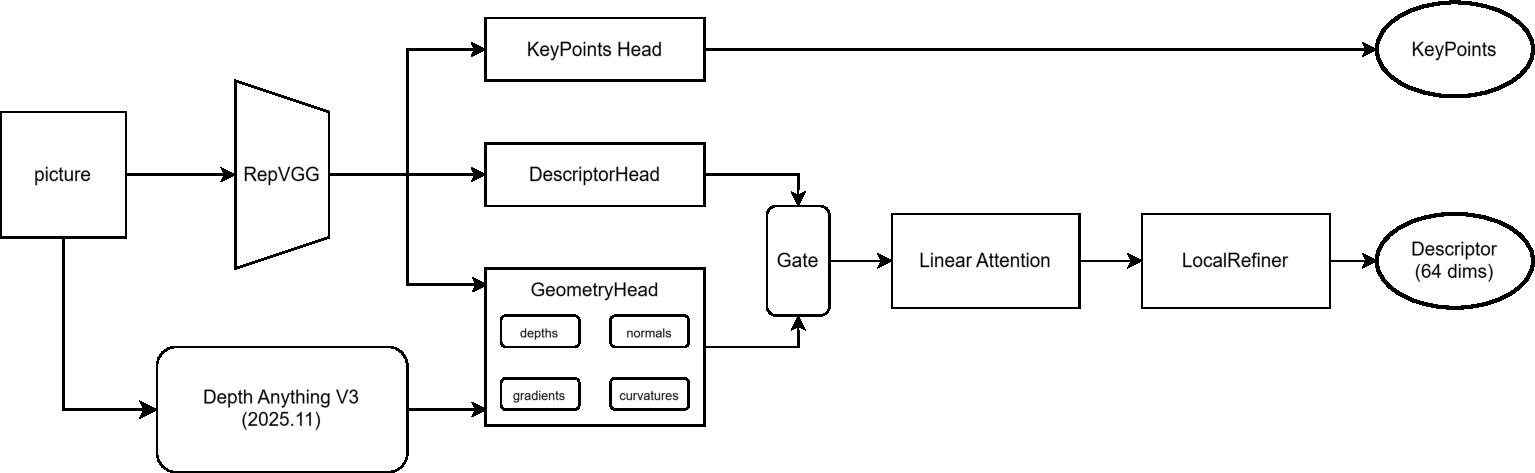
\includegraphics[width=0.9\textwidth]{./img/CurrentModel.pdf}
			\caption{GeoFeat framework overview.}
			\label{fig:GeoFeat}
		\end{figure}
		\par 如图\ref{fig:GeoFeat}所示，GeoFeat 的主干网络支持 Standard CNN 与 RepVGG 两种配置。输入图像首先转换为灰度并进行归一化，随后经五层卷积块提取多尺度特征。我们融合 $x_3, x_4, x_5$ 三层特征，兼顾局部纹理细节与高层语义上下文。关键点分支输出 65 通道 logits（$8\times8$ 栅格位置加背景），描述子分支输出稠密特征图。
		\par 几何分支使用几何头预测多通道几何图，并根据配置动态选择深度、法向量、梯度与曲率分量。之后在 FeatureBooster 中分别执行描述子编码和几何编码，再通过全局交互模块与局部细化模块进行融合。最终描述子经过 $L_2$ 归一化输出，同时利用 repeatability map 调整关键点 logits。
	\subsection{Multi-order Geometric Representation}
		\par 给定深度图 $D \in \mathbb{R}^{H\times W}$，我们先计算一阶导数 $D_x,D_y$ 与二阶导数 $D_{xx},D_{yy},D_{xy}$。法向量定义为
		\begin{equation}
		\mathbf{n}=\frac{(-D_x,-D_y,1)}{\|(-D_x,-D_y,1)\|_2}.
		\end{equation}
		主曲率通过 Hessian 的特征值近似：
		\begin{equation}
		k_{1,2}=\frac{\mathrm{tr}(\mathbf{H})\pm\sqrt{\mathrm{tr}(\mathbf{H})^2-4\det(\mathbf{H})}}{2},
		\end{equation}
		其中 $\mathrm{tr}(\mathbf{H})=D_{xx}+D_{yy}$，$\det(\mathbf{H})=D_{xx}D_{yy}-D_{xy}^2$。
		\begin{figure}[ht]
			\centering
			\setlength{\tabcolsep}{0pt}
			\begin{tabular}{cccc}
				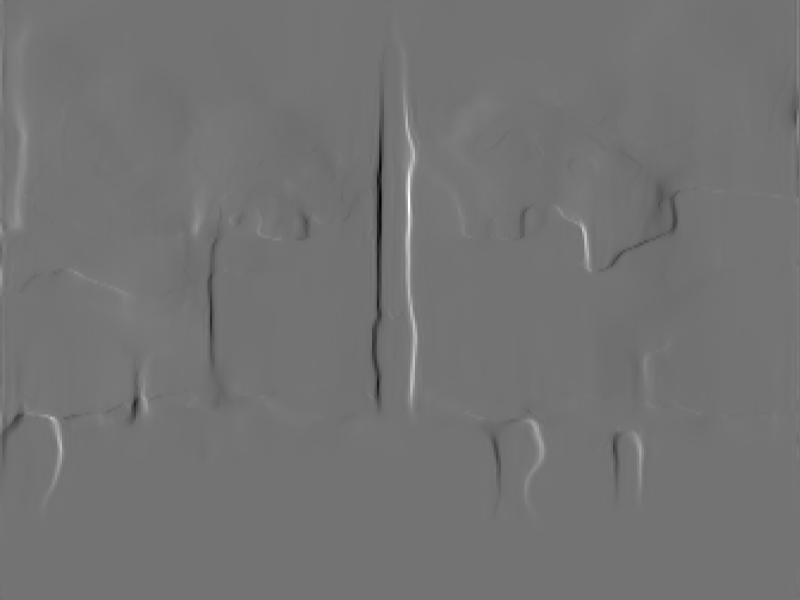
\includegraphics[width=0.24\textwidth,height=0.16\textwidth]{./img/scence1_grad_x.png} &
				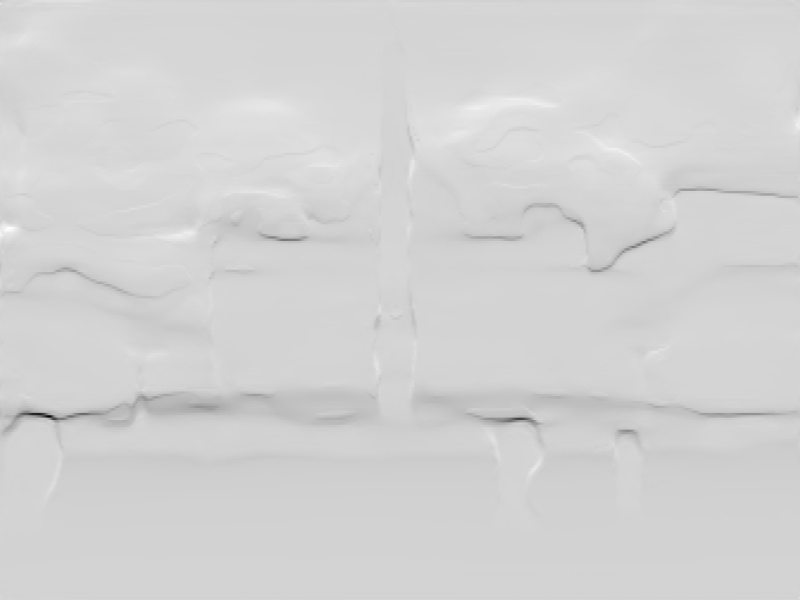
\includegraphics[width=0.24\textwidth,height=0.16\textwidth]{./img/scence1_grad_y.png} &
				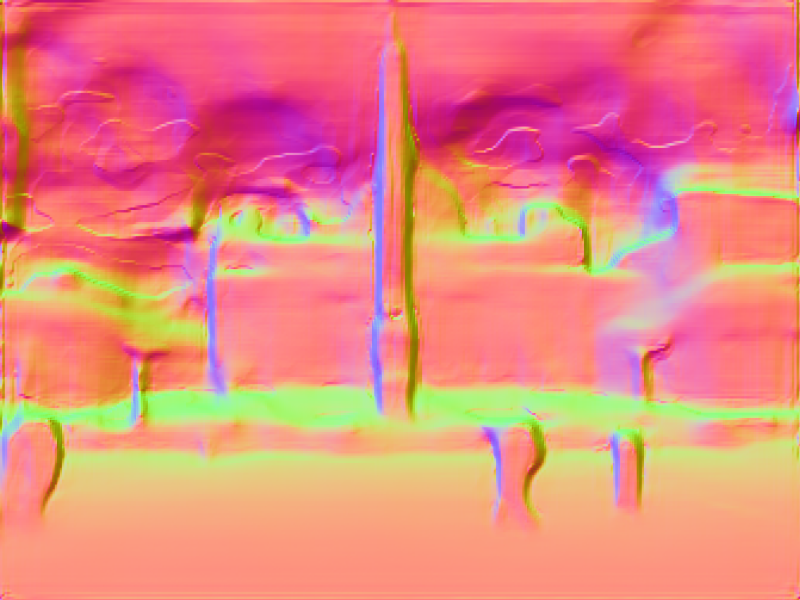
\includegraphics[width=0.24\textwidth,height=0.16\textwidth]{./img/scence1_norm.png} &
				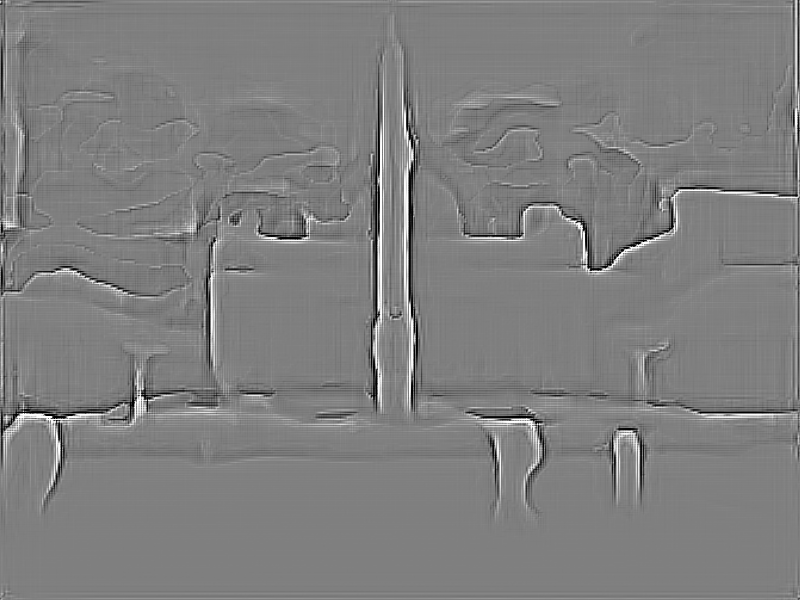
\includegraphics[width=0.24\textwidth,height=0.16\textwidth]{./img/scence1_curv_H.png} \\[-5pt]
				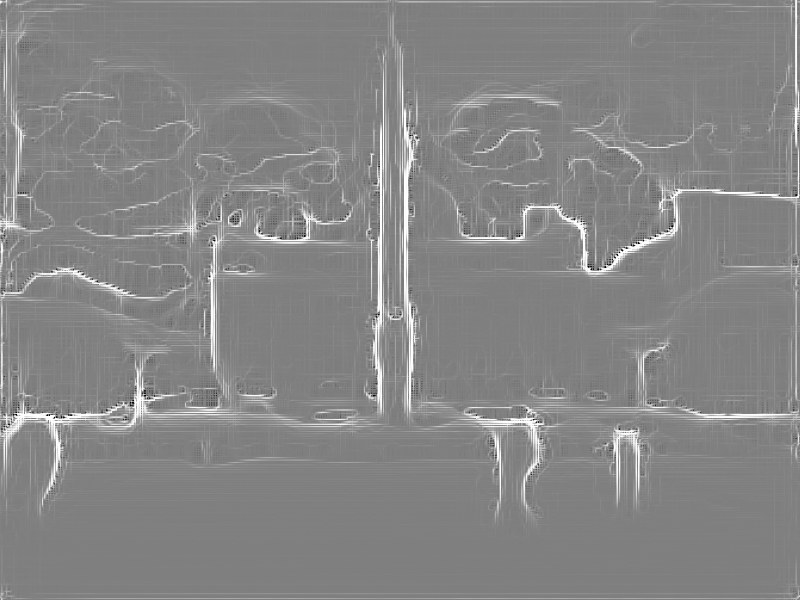
\includegraphics[width=0.24\textwidth,height=0.16\textwidth]{./img/scence1_curv_k1.png} &
				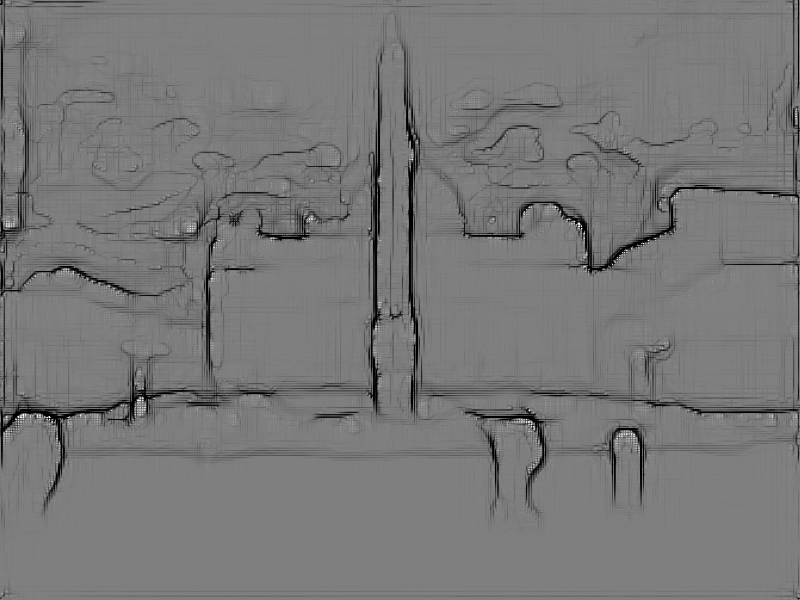
\includegraphics[width=0.24\textwidth,height=0.16\textwidth]{./img/scence1_curv_k2.png} &
				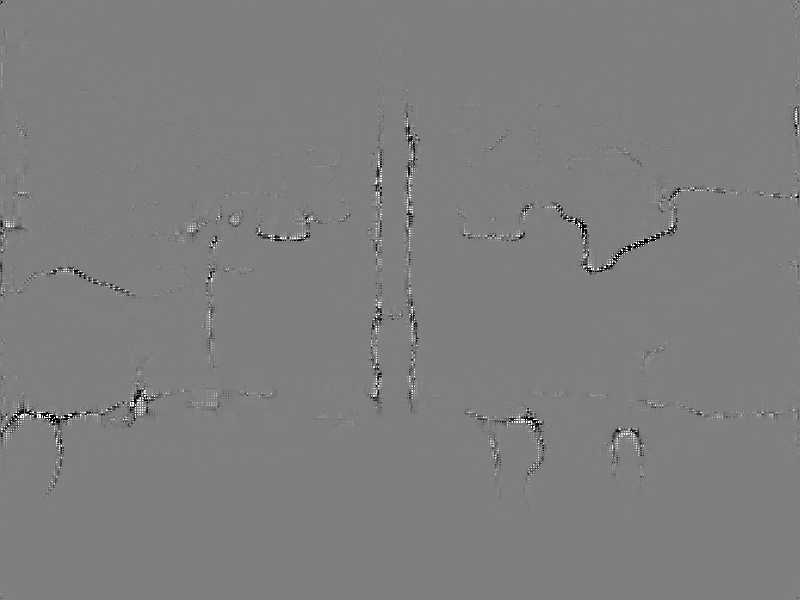
\includegraphics[width=0.24\textwidth,height=0.16\textwidth]{./img/scence1_curv_K.png} &
				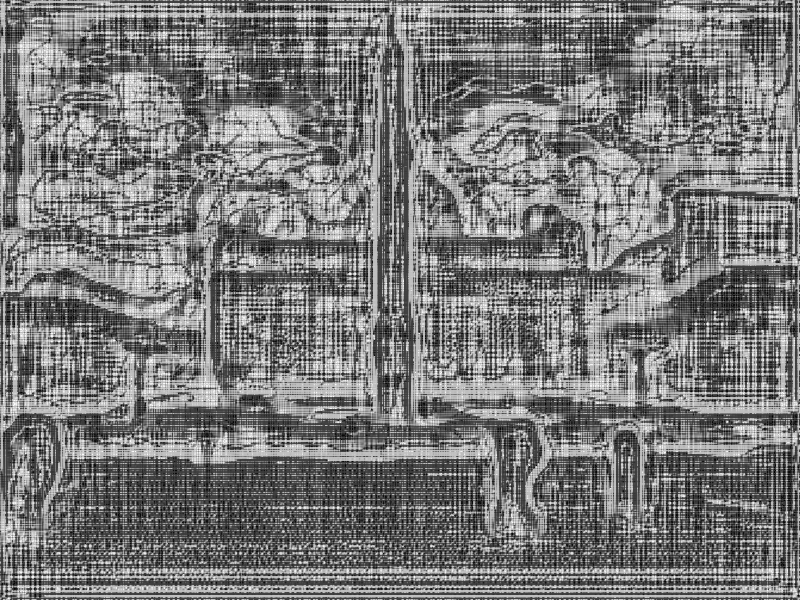
\includegraphics[width=0.24\textwidth,height=0.16\textwidth]{./img/scence1_curv_SI.png}
			\end{tabular}
			\caption{Example geometric maps: gradients, normals, and curvature channels.}
		\end{figure}

		\par 从可视化结果可以观察到，不同几何通道对结构信息具有互补响应。梯度图中，$D_x$ 主要强化垂直边界，$D_y$ 主要强化水平边界，能够稳定突出深度突变位置；法向量图在大面积平面区域呈现较高一致性，而在物体边界与表面朝向突变处出现明显变化，反映了局部朝向不连续性。
		\par 需要说明的是，尽管几何计算模块可以同时得到主曲率 $k_1,k_2$、高斯曲率 $K$、平均曲率 $H_m$ 与形状指数等量，但当前网络实现仅将曲率分支作为单通道输入，并在训练阶段以平均曲率 $H_m$ 作为监督目标。这样设计的原因有三点：第一，现有主干融合接口对曲率分支的通道预算为 1，直接引入多通道曲率会改变模型结构与参数规模；第二，$k_1,k_2,K$ 和形状指数对深度噪声更敏感。当 $k_1 = k_2$ 时，该点称为曲面\textbf{脐点}（umbilic point）：曲面在该点所有切方向上的法曲率相等，不存在可区分的主方向，局部呈现均匀的"球面型"或"平坦型"弯曲（球面上每一点、大面积平坦壁面均属此类）。形状指数定义为
		\begin{equation}
		\mathrm{SI} = \frac{2}{\pi}\arctan\frac{k_1+k_2}{k_2-k_1},
		\end{equation}
		其分母恰为 $k_2 - k_1$。在脐点处 $k_2 - k_1 = 0$，形状指数产生数值奇异；即使仅存在微小深度噪声扰动，分母也可急剧趋近于零，导致形状指数对噪声极度敏感。训练中这类不稳定高频响应容易被放大，而 $H_m$ 在边界与曲面过渡区域仍保留主要几何信息且更平滑；第三，本工作目标是轻量化部署，使用单通道曲率可在计算开销与几何约束效果之间取得更稳健的折中。因此，本文将其余曲率量用于几何分析与可视化，不作为当前版本模型的直接训练输入。
		\par 在实现中，梯度分支使用 2 通道 $(D_x,D_y)$，法向量分支使用 3 通道，深度分支使用 1 通道；曲率分支在主干融合时采用 1 通道表示。虽然几何计算模块可导出 $k_1,k_2,K,H_m$ 与形状指数等量，但当前训练中的曲率监督项对齐的是平均曲率 $H_m$。因此，当前 GeoFeat 的几何输入通道配置为 depth(1) + normal(3) + gradients(2) + curvature(1)。
	\subsection{Global-Local Geometric Fusion}
		\par 为在效率与表达能力间取得平衡，我们采用两级融合策略：
		\begin{itemize}
		\item \textbf{Global interaction:} 使用 attention-free 结构进行全局上下文建模，避免传统自注意力的高计算开销。
		\item \textbf{Local refinement:} 当启用 GCLA 时，视觉分支与几何分支分别执行多尺度深度可分离卷积，并通过跨模态门控实现双向耦合，增强边缘与结构不连续区域的描述稳定性。
		\end{itemize}
	\subsection{Training Objectives}
		\par 总损失由描述子匹配、关键点蒸馏与几何一致性项构成：
		\begin{equation}
		\mathcal{L}=\lambda_d\mathcal{L}_{desc}+\lambda_f\mathcal{L}_{fb}+\lambda_k\mathcal{L}_{kpt}+\lambda_h\mathcal{L}_{heat}+\lambda_g\mathcal{L}_{geo}.
		\end{equation}
		其中，$\mathcal{L}_{desc}$ 与 $\mathcal{L}_{fb}$ 使用双向概率匹配约束描述子一致性；$\mathcal{L}_{kpt}$ 使用蒸馏监督约束关键点响应；$\mathcal{L}_{geo}$ 对深度、梯度与曲率分支施加一致性约束。在当前实现里，曲率损失项使用单通道预测与目标平均曲率 $H_m$ 的 $L_1$ 约束。该联合目标提升了模型在复杂场景中的匹配稳定性。
	\section{Experiments}
		\par 训练实现基于 PyTorch Lightning，采用 COCO 增强样本与 MegaDepth 样本混合训练。优化器使用 Adam，初始学习率设为 $3\times10^{-4}$，并使用阶梯衰减策略。输入分辨率设置为 $800\times600$，损失项权重采用联合调参策略。
		\par 评估采用 MegaDepth1500 协议，以位姿估计误差统计 AUC 指标。根据当前仓库评估记录，baseline2 配置在该流程下可获得稳定结果（例如 AUC@5/@10/@20 约为 45.04/59.00/70.27）。这些结果验证了 GeoFeat 设计在复杂几何场景下的有效性，并为后续 GCLA 与 no-unfold 等结构消融提供了对照基线。
		\par 我们建议在最终稿中补充三类消融：
		\begin{itemize}
		\item 几何阶数消融：深度、深度+法向量、深度+法向量+梯度、全量多阶几何；
		\item 融合模块消融：无局部细化、LocalRefiner、GCLA；
		\item 预处理模式消融：unfold 与 no\_unfold\_lite。
		\end{itemize}
	\section{Conclusion}
		\par 本文提出 GeoFeat，一种面向局部特征匹配的轻量级几何增强框架。GeoFeat 将多阶几何信息显式引入描述子学习流程，并通过注意力自由全局建模与几何耦合局部聚合实现高效融合。在联合损失约束下，模型能够在复杂场景中获得更稳定的匹配性能。未来工作将进一步探索跨域自适应几何蒸馏与实时部署优化，以提升在动态场景与低算力平台上的泛化能力。

\bibliographystyle{IEEEtran}
\bibliography{references}
\end{document}